% !TeX spellcheck = cs_CZ
{\tikzset{external/prefix={tikz/FYZII/}}
 \tikzset{external/figure name/.add={ch23_}{}}
%---------------------------------------------------------------------------------------------------
% file fey2ch23.tex
%---------------------------------------------------------------------------------------------------
%====================Kapitola: Dutinové rezonátory =================================================
\chapter{Dutinové rezonátory}\label{fyz:IIchapXXIII}
\minitoc
\section{Reálné prvky obvodů}\label{fyz:IIchapXXIIIsecI}
\section{Kondenzátor při vysokch frekvencích}\label{fyz:IIchapXXIIIsecII}
\section{Rezonanční dutina}\label{fyz:IIchapXXIIIsecIII}
\section{Kmitavé mody dutinových rezonátorů}\label{fyz:IIchapXXIIIsecIV}
\section{Dutinové rezonátory a rezonanční obvody}\label{fyz:IIchapXXIIIsecV}

    \begin{figure}[ht!] %\ref{fyz_fig583}
      \centering
      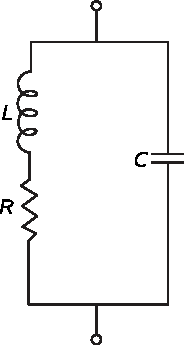
\includegraphics[width=0.3\linewidth]{fyz_fig583.pdf}
      \caption{
               (\cite[s.~707]{Feynman02})}
      \label{fyz_fig583}
    \end{figure}

    \begin{figure}[ht!]
      \centering
      \begin{tabular}{cc}
        \subfloat[ ]{\label{fyz_fig584a}
          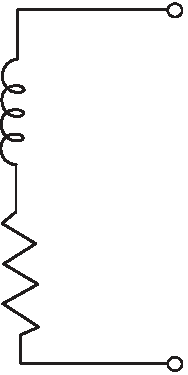
\includegraphics[width=0.3\linewidth]{fyz_fig584a.pdf}}               &
        \subfloat[ ]{\label{fyz_fig584b}
          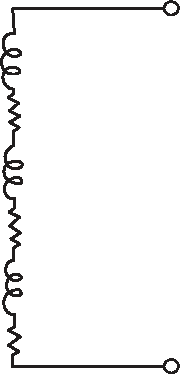
\includegraphics[width=0.3\linewidth]{fyz_fig584b.pdf}}
      \end{tabular}
      \label{fyz_fig584}
      \caption{
               (\cite[s.~748]{Feynman02})}
    \end{figure}
    
    \begin{figure}[ht!]
      \centering
      \begin{tabular}{ccc}
        \subfloat[ ]{\label{fyz_fig585a}
          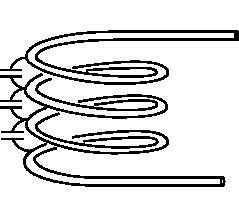
\includegraphics[width=0.3\linewidth]{fyz_fig585a.pdf}}               &
        \subfloat[ ]{\label{fyz_fig585b} 
          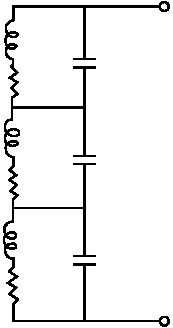
\includegraphics[width=0.3\linewidth]{fyz_fig585b.pdf}}               &
        \subfloat[ ]{\label{fyz_fig585c}
          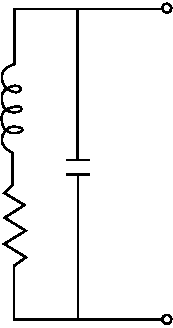
\includegraphics[width=0.3\linewidth]{fyz_fig585c.pdf}}
      \end{tabular}
      \label{fyz_fig585}
      \caption{
               (\cite[s.~748]{Feynman02})}
    \end{figure}

    \begin{figure}[ht!] %\ref{fyz_fig586}
      \centering
      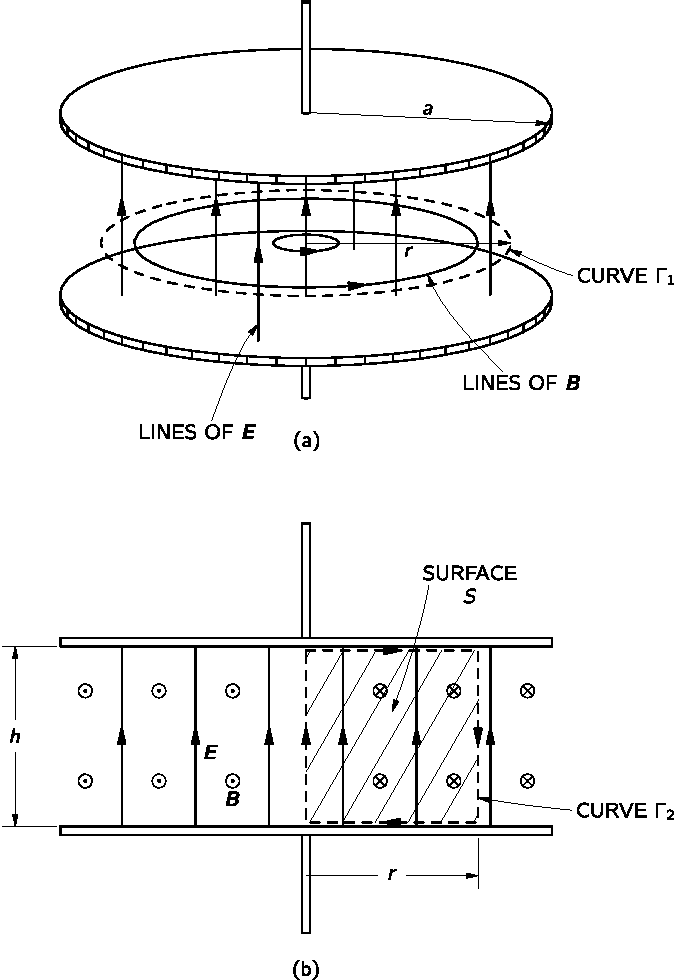
\includegraphics[width=0.7\linewidth]{fyz_fig586.pdf}
      \caption{
               (\cite[s.~707]{Feynman02})}
      \label{fyz_fig586}
    \end{figure}
    
    \begin{figure}[ht!] %\ref{fyz_fig587}
      \centering
      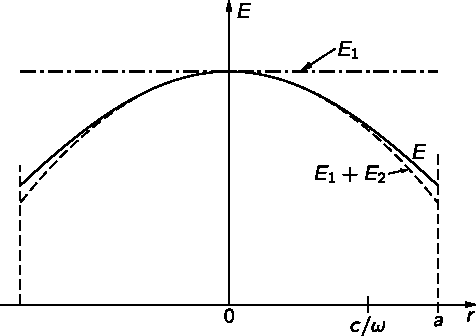
\includegraphics[width=0.7\linewidth]{fyz_fig587.pdf}
      \caption{
               (\cite[s.~707]{Feynman02})}
      \label{fyz_fig587}
    \end{figure}

    \begin{figure}[ht!] %\ref{fyz_fig588}
      \centering
      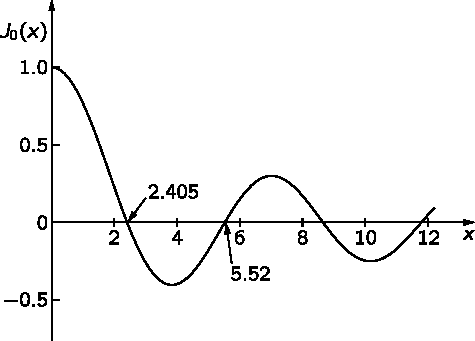
\includegraphics[width=0.7\linewidth]{fyz_fig588.pdf}
      \caption{
               (\cite[s.~707]{Feynman02})}
      \label{fyz_fig588}
    \end{figure}

    \begin{figure}[ht!]
      \centering
      \begin{tabular}{c}
        \subfloat[ ]{\label{fyz_fig589a}
          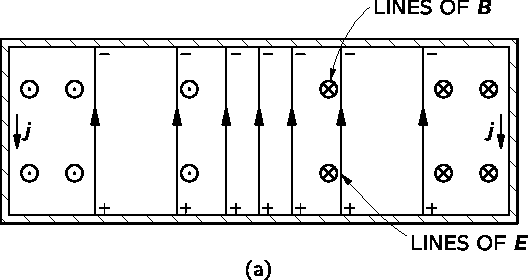
\includegraphics[width=0.7\linewidth]{fyz_fig589a.pdf}}               \\
        \subfloat[ ]{\label{fyz_fig589b}
          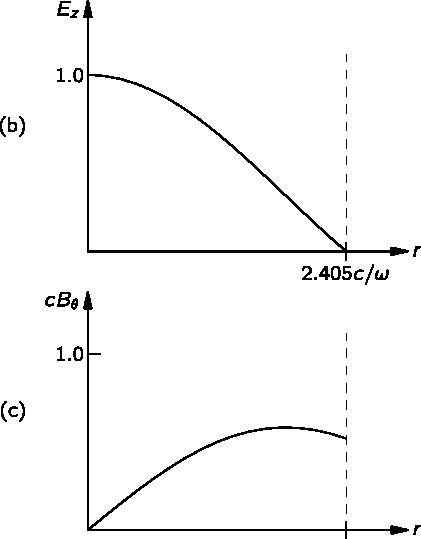
\includegraphics[width=0.7\linewidth]{fyz_fig589b.pdf}}              
      \end{tabular}
      \caption{Pohyb tekutiny v proudové trubici
               (\cite[s.~748]{Feynman02})}
    \end{figure}

    \begin{figure}[ht!] %\ref{fyz_fig590}
      \centering
      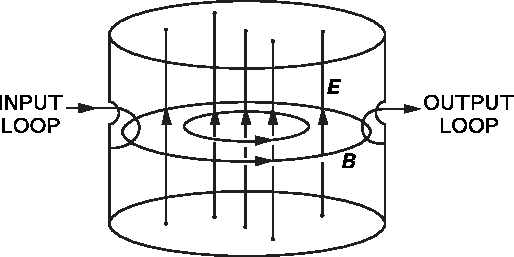
\includegraphics[width=0.7\linewidth]{fyz_fig590.pdf}
      \caption{
               (\cite[s.~707]{Feynman02})}
      \label{fyz_fig590}
    \end{figure}
    
    \begin{figure}[ht!] %\ref{fyz_fig591}
      \centering
      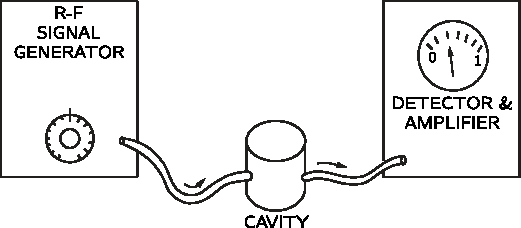
\includegraphics[width=0.7\linewidth]{fyz_fig591.pdf}
      \caption{
               (\cite[s.~707]{Feynman02})}
      \label{fyz_fig591}
    \end{figure}

    \begin{figure}[ht!] %\ref{fyz_fig592}
      \centering
      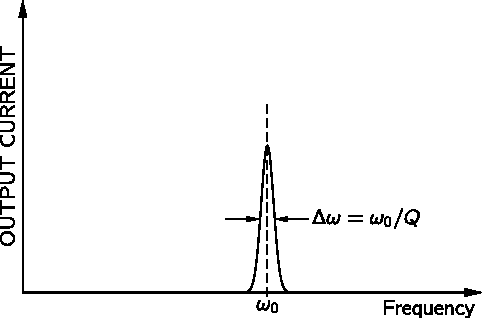
\includegraphics[width=0.7\linewidth]{fyz_fig592.pdf}
      \caption{
               (\cite[s.~707]{Feynman02})}
      \label{fyz_fig592}
    \end{figure}

    \begin{figure}[ht!] %\ref{fyz_fig593}
      \centering
      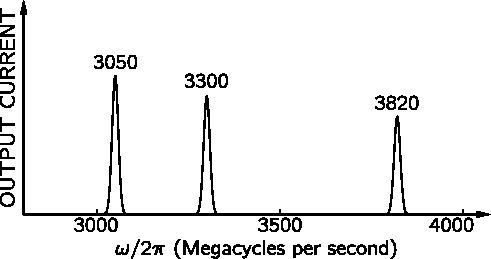
\includegraphics[width=0.7\linewidth]{fyz_fig593.pdf}
      \caption{
               (\cite[s.~707]{Feynman02})}
      \label{fyz_fig593}
    \end{figure}

    \begin{figure}[ht!]
      \centering
      \begin{tabular}{c}
        \subfloat[ ]{\label{fyz_fig594a}
          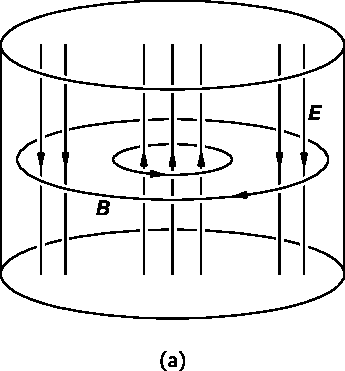
\includegraphics[width=0.5\linewidth]{fyz_fig594a.pdf}}               \\
        \subfloat[ ]{\label{fyz_fig594b}
          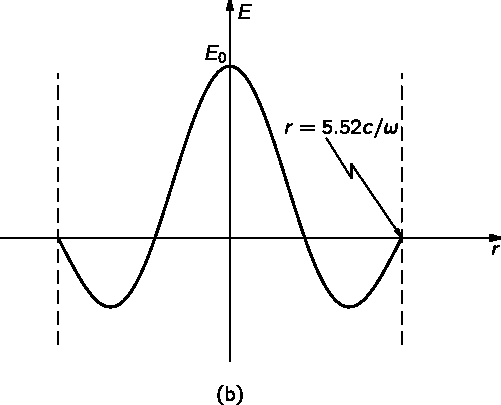
\includegraphics[width=0.5\linewidth]{fyz_fig594b.pdf}}              
      \end{tabular}
      \caption{
               (\cite[s.~748]{Feynman02})}
    \end{figure}

    \begin{figure}[ht!] %\ref{fyz_fig595}
      \centering
      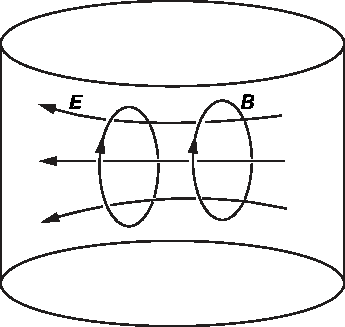
\includegraphics[width=0.5\linewidth]{fyz_fig595.pdf}
      \caption{
               (\cite[s.~707]{Feynman02})}
      \label{fyz_fig595}
    \end{figure}

    \begin{figure}[ht!] %\ref{fyz_fig596}
      \centering
      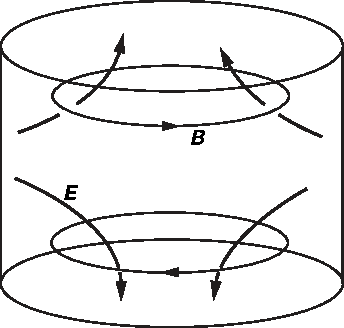
\includegraphics[width=0.5\linewidth]{fyz_fig596.pdf}
      \caption{
               (\cite[s.~707]{Feynman02})}
      \label{fyz_fig596}
    \end{figure}

    \begin{figure}[ht!]
      \centering
      \begin{tabular}{c}
        \subfloat[ ]{\label{fyz_fig597a}
          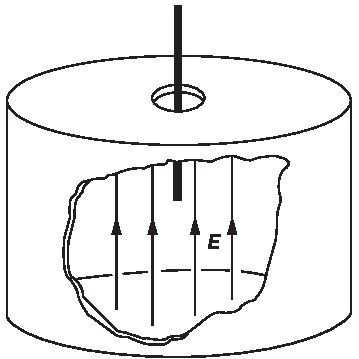
\includegraphics[width=0.5\linewidth]{fyz_fig597a.pdf}}               \\
        \subfloat[ ]{\label{fyz_fig597b}
          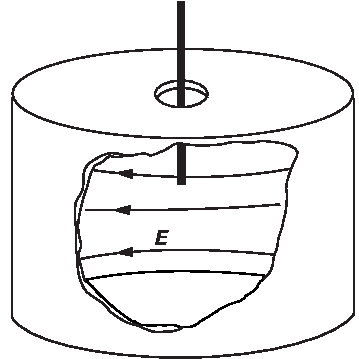
\includegraphics[width=0.5\linewidth]{fyz_fig597b.pdf}}               \\
        \subfloat[ ]{\label{fyz_fig597c}
          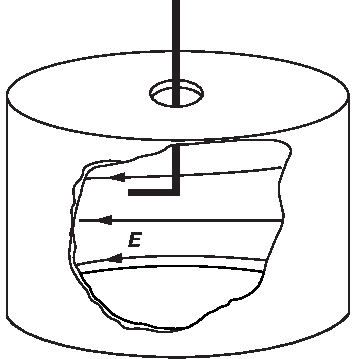
\includegraphics[width=0.5\linewidth]{fyz_fig597c.pdf}}
      \end{tabular}
      \label{fyz_fig597}
      \caption{
               (\cite[s.~748]{Feynman02})}
    \end{figure}

    \begin{figure}[ht!]
      \centering
      \begin{tabular}{c}
        \subfloat[ ]{\label{fyz_fig598a}
          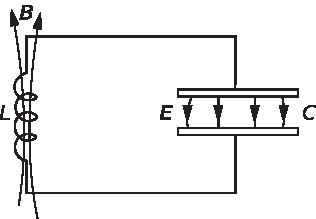
\includegraphics[width=0.6\linewidth]{fyz_fig598a.pdf}}               \\
        \subfloat[ ]{\label{fyz_fig598b}
          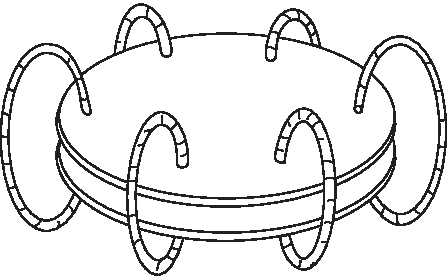
\includegraphics[width=0.6\linewidth]{fyz_fig598b.pdf}}               \\
        \subfloat[ ]{\label{fyz_fig598c}
          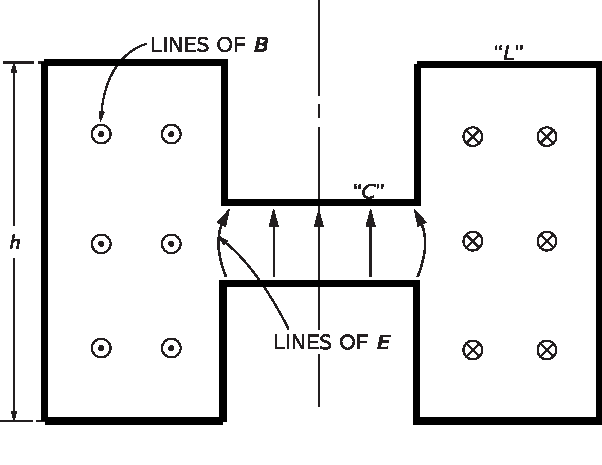
\includegraphics[width=0.7\linewidth]{fyz_fig598c.pdf}}
      \end{tabular}
      \label{fyz_fig598}
      \caption{
               (\cite[s.~748]{Feynman02})}
    \end{figure}

    \begin{figure}[ht!] %\ref{fyz_fig599}
      \centering
      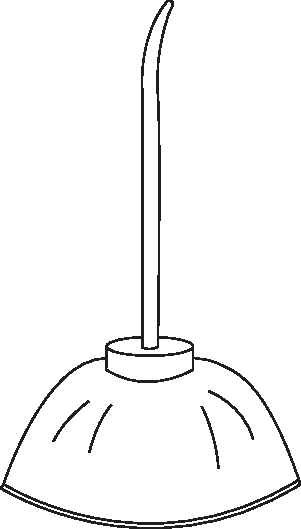
\includegraphics[width=0.3\linewidth]{fyz_fig599.pdf}
      \caption{
               (\cite[s.~707]{Feynman02})}
      \label{fyz_fig599}
    \end{figure}

} %tikzset
%~~~~~~~~~~~~~~~~~~~~~~~~~~~~~~~~~~~~~~~~~~~~~~~~~~~~~~~~~~~~~~~~~~~~~~~~~~~~~~~~~~~~~~~~~~~~~~~~~~
\printbibliography[title={Seznam literatury}, heading=subbibliography]
\addcontentsline{toc}{section}{Seznam literatury}